\subsubsection{\emph{Development View}}
\label{subsubsec:development-view}

\begin{figure}[htbp]
    \centering
    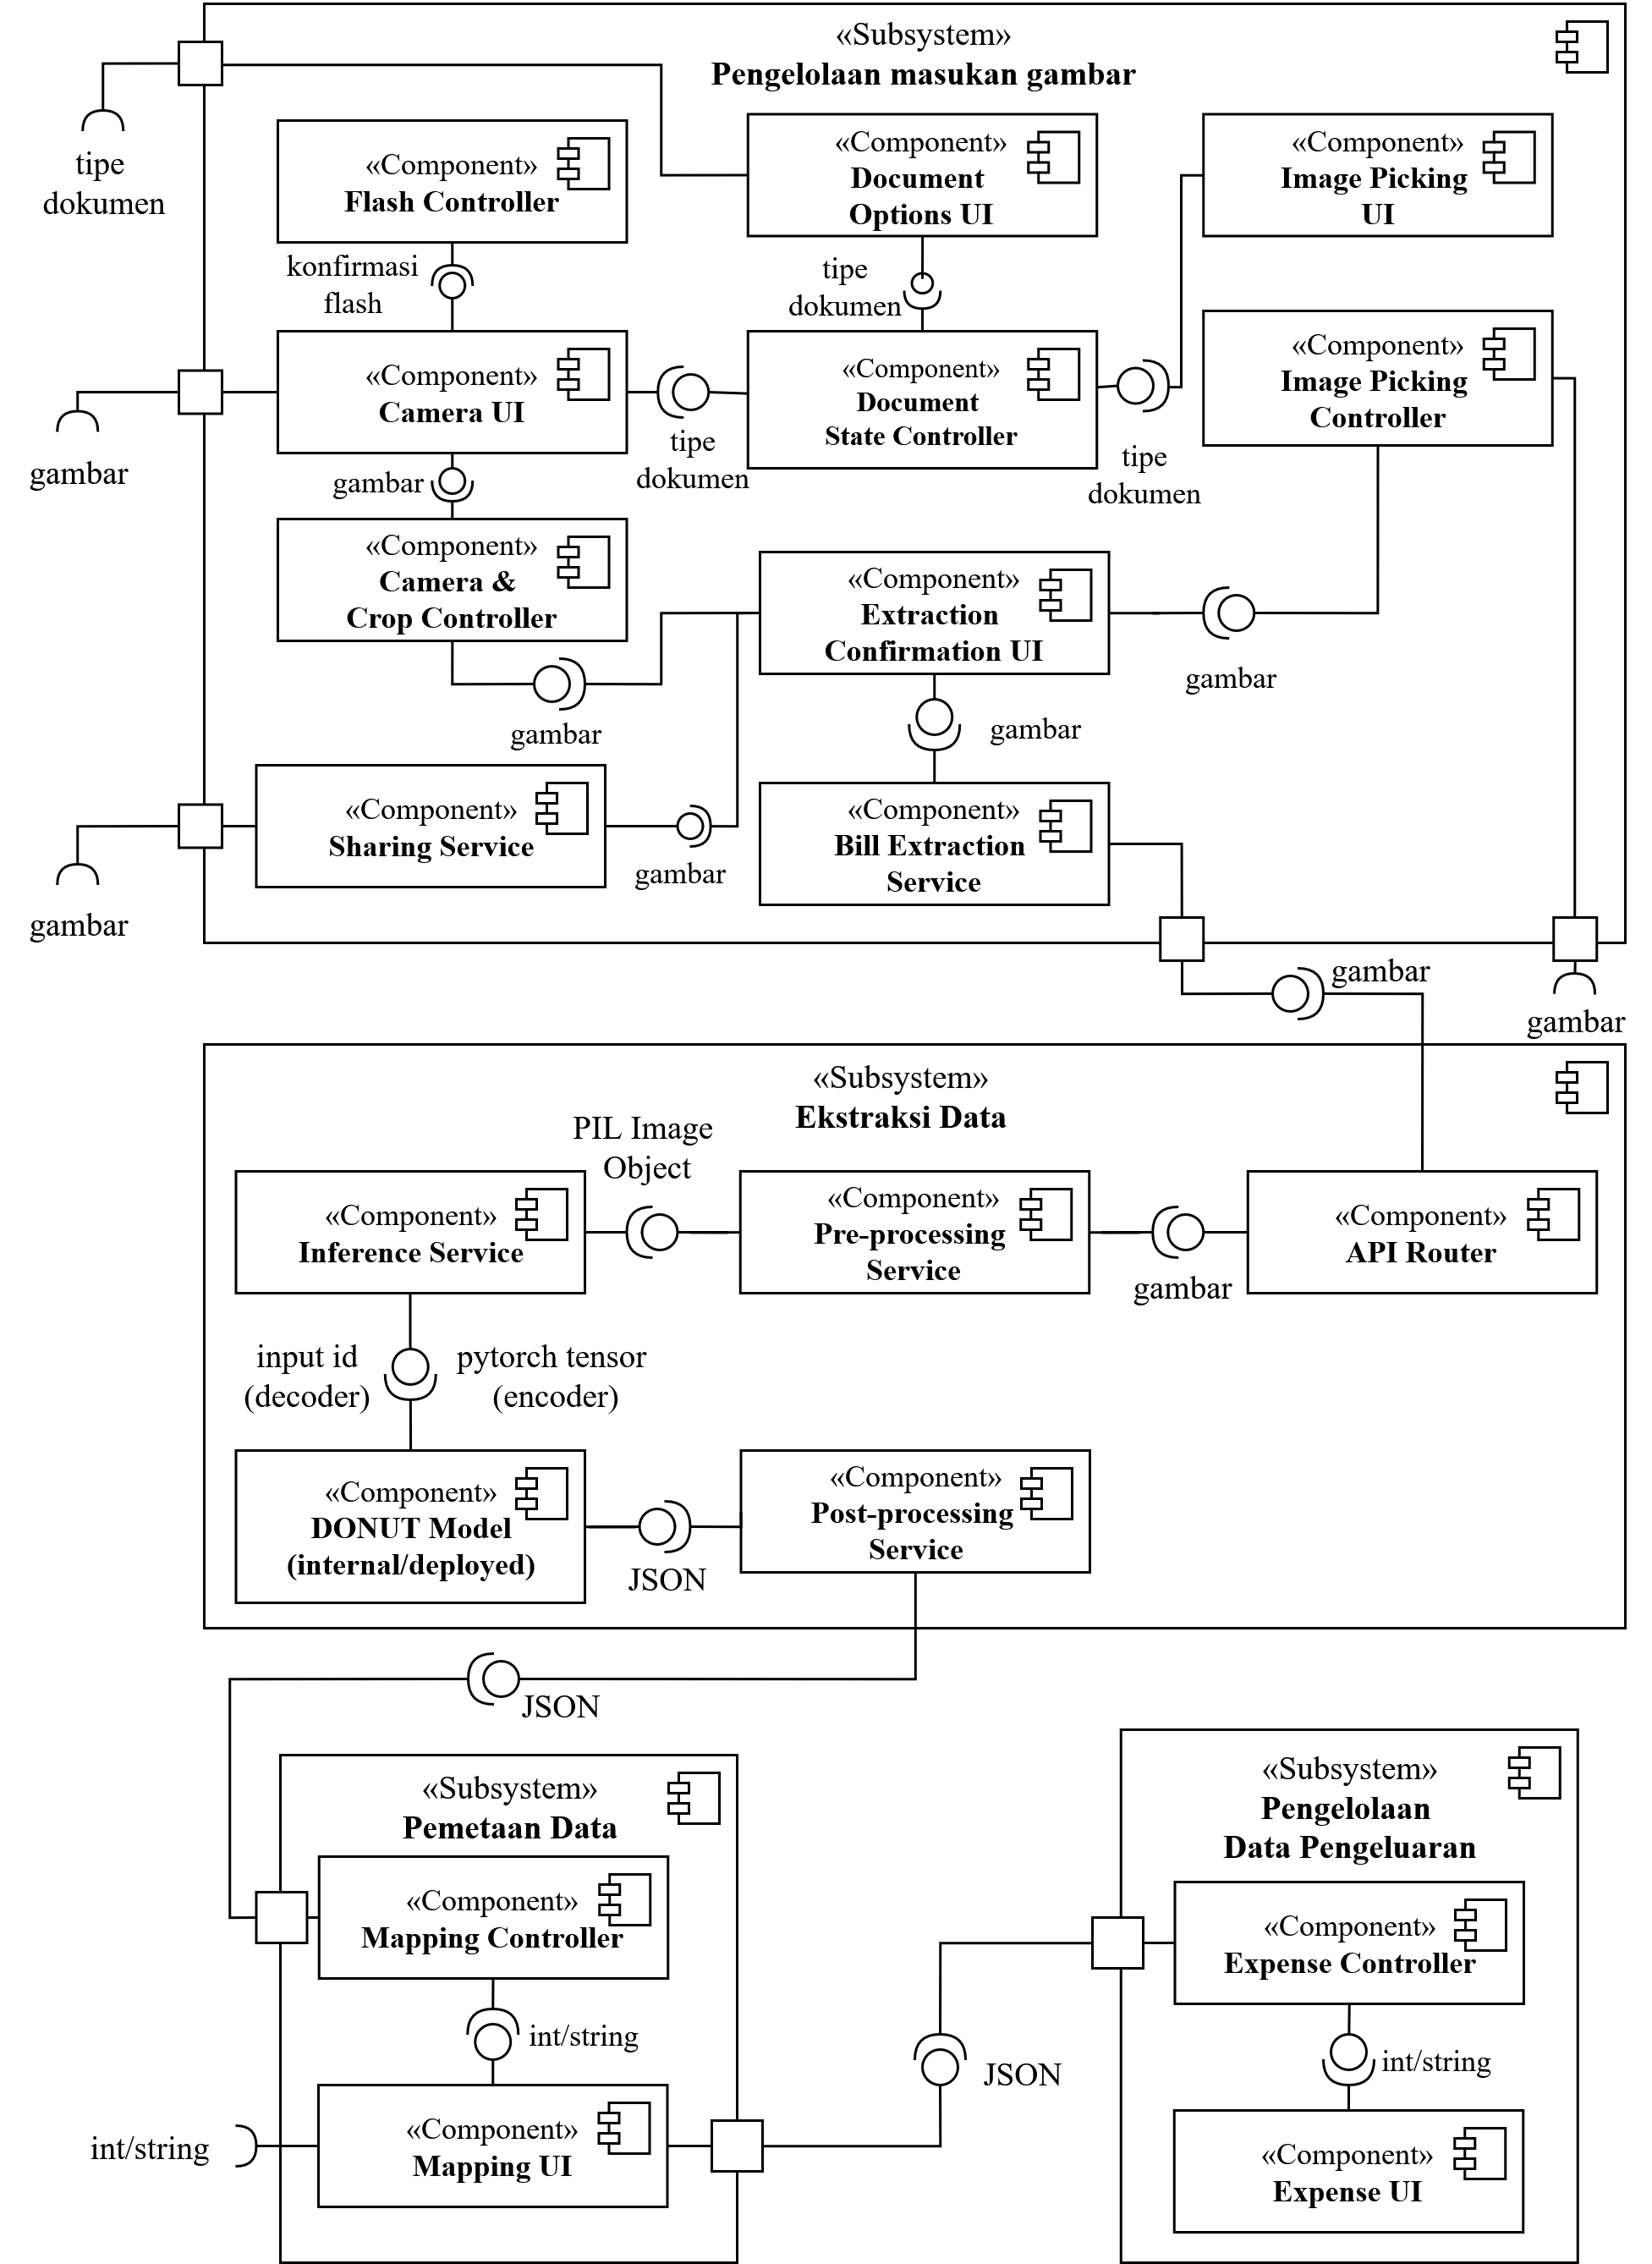
\includegraphics[width=1\textwidth]{images/component-diagram.png}
    \caption{\emph{Component diagram} sistem pencatatan pengeluaran berbasis \emph{mobile}}
    \label{fig:component-diagram}
\end{figure}

\emph{Development view} mendefinisikan organisasi sistem dari sudut pandang pengembang. \emph{Development view} membuat pengembang dapat memahami struktur sistem hingga level komponen dan bagaimana komponen tersebut berinteraksi satu sama lain. \autoref{fig:component-diagram} menunjukkan \emph{component diagram} sistem pencatatan pengeluaran berbasis \emph{mobile}. Diagram ini menunjukkan bagaimana sistem dibagi menjadi beberapa komponen, yaitu aplikasi \emph{mobile}, layanan \emph{backend}, model internal, dan model \emph{deployed}. Setiap komponen memiliki tanggung jawab dan interaksi yang jelas dengan komponen lainnya untuk memungkinkan pengembangan sistem yang lebih terstruktur.

Sistem terbagi menjadi empat subsistem utama, yaitu subsistem pengelolaan masukan gambar, subsistem ekstraksi data, subsistem pemetaan data, dan subsistem pengelolaan data pengeluaran. Setiap subsistem memiliki tanggung jawab yang berbeda dan berinteraksi satu sama lain untuk mencapai tujuan sistem secara keseluruhan. Subsistem pengelolaan masukan gambar bertanggung jawab untuk menerima dan memproses gambar bukti pembayaran yang diunggah oleh pengguna dan mengirimkannya ke subsistem ekstraksi data untuk kemudian diolah. Masukan gambar dapat berasal dari tangkapan kamera, pengunggahan gambar, dan metode "Sharing" dari sistem operasi terkait. 

Subsistem ekstraksi data bertanggung jawab untuk mengekstrak informasi penting dari gambar bukti pembayaran menggunakan model \donut{} sesuai dengan jenis dokumen yang diunggah. Hasil inferensi dari model  akan mengolah diolah informasi terstruktur dalam format JSON. Data terstruktur tersebut akan dikirimkan ke subsistem pemetaan data untuk dipetakan agar dapat dilihat oleh pengguna. Subsistem pemetaan data mengonfirmasi hasil ekstraksi kepada pengguna. Dengan konfirmasi pengguna, subsistem akan mengirimkan hasil ekstraksi data ke subsistem pengelolaan data pengeluaran. Subsistem pengelolaan data pengeluaran bertanggung jawab untuk menyimpan, mengelola, dan menampilkan data pengeluaran kepada pengguna saat pengguna ingin melihat total pengeluaran mereka.